\chapter{Theory}
This experiment explores the electrical behavior of various conductors and semiconductors at cryogenic temperatures.

\section{Metals}

\subsection{Classical Electrical Conductivity}
The classical concept of free, localized electrons gives a simple explanation for electrical resistance, assuming that the electrons can scatter on the nuclei of the conductor material.
An external electric field $E$ accelerates the electrons with mass $m$, which regularly lose their kinetic energy to elastic collisions with nuclei.
The mean time between collisions $\tau$ depends on the parameters of the conductor's lattice structure.
Solving the equations of motion gives the term
\begin{equation*}
	\frac{m}{\tau} v_\text{D} = - e E
\end{equation*}
for the mean drift velocity $v_\text{D}$. The current density $j$ is given by $j = - e n v_\text{D}$, where $n$ denotes the density of electrons.
Using the definition of the conductance $j = \sigma E$ yields
\begin{equation}\label{eq:classical-resistance}
	\sigma = \frac{n e^2 \tau}{m}.
\end{equation}

\subsection{Temperature Dependence}
Most materials show a dependence on temperature in their electrical properties.
The density of free electrons $n$ in metals is independent of temperature, so the dependency must be in $\tau$, as the other variables in the RHS of \autoref{eq:classical-resistance} are constants.

In addition to the nuclei, electrons can also scatter on lattice defects and, more importantly, phonons, which are strongly associated with temperature.
The scattering processes are independent of each other, the total scattering rate $\tau^{-1}$ is calculated as the sum of the scattering rates due to phonons $\tau_\text{ph}^{-1}$ and nuclei/defects $\tau_\text{de}^{-1}$
\begin{equation*}
	\frac{1}{\tau} = \frac{1}{\tau_\text{ph}} + \frac{1}{\tau_\text{de}}.
\end{equation*}
Similarly, the specific resistance $\rho$ can be written as
\begin{equation*}
	\rho = \rho_\text{ph}(T) + \rho_\text{de},
\end{equation*}
the temperature independent $\rho_\text{de}$ is also called residual resistance, as it persists even at low temperatures, where phonon scattering is suppressed.

An exact term for $\rho_\text{ph}(T)$, calculated by Grüneisen \cite{elresistancemetal}, is given by
\begin{equation}
	\rho_\text{ph}(T) = A \left(\frac{T}{\Theta}\right)^5 \cdot \int_0^\frac{\Theta}{T}\frac{x^5}{(\e^x - 1)(1 - \e^{-x})} \d x,
\end{equation}
where $\Theta$ denotes the debye temperature and $A$ is a material dependent constant.
For low temperatures $T \ll \Theta$ this function behaves like $T^5$, for higher $T$ a linear behavior emerges.

The resistance of a sample can be split up like the specific resistance as
\begin{equation*}
	R = R_\text{res} + R_\text{T}(T),
\end{equation*}
where $R_\text{res}$ denotes the residual resistance.

In the linear region the resistance approaches \cite{elresistancemetal}
\begin{equation}
	R_\text{T}(T) = \num{1.17} \cdot \frac{R_\Theta}{\theta} \cdot T - \num{0.17} \cdot R_\Theta,
\end{equation}
where $R_\Theta$ is the resistance at the debye temperature $\Theta$ (at least we think it does, the article is behind a paywall).
This facilitates a straightforward way to measure the debye temperature.

\section{Semiconductors}
Semiconductors are materials with a Fermi level inside their band gap at equilibrium, where the band gap is significantly smaller than that of an insulator.
Two types of semiconductors may be distinguished: intrinsic semiconductors which have their Fermi level right in the middle of the band gap and extrinsic materials which are also referred to as 'doped'.

\subsection{Doping}
A pure semiconductor is not very useful, since it is neither a good insulator, nor a good conductor.
By adding impurities to or gating pure semiconductors (such as pure Si) their electrical properties may be varied in a useful manner.
Doping and gating draw either the conduction or the valence band very close to the Fermi level, greatly increasing the number of free states there.

Doping is accomplished by adding small quantities of foreign atoms to the semiconductor.
Consider for example Si from the fourth main group of the periodic system of elements which has four valence electrons that bond each silicon atom to its neighbors.
Adding either elements from the third (i.e. B, In) or fifth main group (i.e. As, P) may be used for creating p- or n-doped semiconductors, since they either lack or add one electron in their valence shells.

In \textit{p-doped} materials the so called \textit{acceptors} leave a vacant electron state (\textit{hole}) when they replace a silicon atom in the crystal.
This hole can move around the lattice and function as a charge carrier.
The acceptor levels have energies just above the valence band.
By supplying a small amount of energy, electrons from the valence band may be excited into these acceptor states and thus ionize the foreign atom, leaving a negatively charged defect behind.

Similarly, in \textit{n-doped} materials the so called \textit{donators} leave one electron free, which can contribute to the conductivity of the material.
These weakly bound electrons have energies just below the conduction band and thus can be excited very easily into conducting states by supplying a small amount of energy.

\subsection{Classical Electrical Conductivity}
The total electrical conductivity is the sum of the individual electron and hole conductivities
\begin{equation*}
	\sigma_\text{tot} = e\left(n_\text{e} \mu_\text{e} + n_\text{h} \mu_\text{h}\right),
\end{equation*}
where $n_\text{i}$ denotes the electron/hole density and $\mu_\text{i}$ is their respective mobility.

For the electrical conductivity of electrons and holes according to the high-temperature limit of Fermi-Dirac statistics it holds
\begin{equation*}
	\sigma_\text{i} = \text{const}\cdot\exp\left(-\frac{E_\text{g}}{2k_\text{B}T}\right),
\end{equation*}
where it is assumed that the considered semiconductor is an ideal, intrinsic semiconductor and $E_\text{g}$ denotes its band gap.

If we now consider a doped semiconductor, the electrical conductivity changes drastically, since we now have to consider impurities.
At high temperatures, phonon scattering contributes to the mobility as
\begin{equation*}
	\mu \propto T^{-\frac{3}{2}}.
\end{equation*}
At low temperatures, the leading contribution is generated by scattering at impurities, invoking a behavior like
\begin{equation*}
	\mu \propto T^{\frac{3}{2}}.
\end{equation*}
\begin{figure}
	\centering
	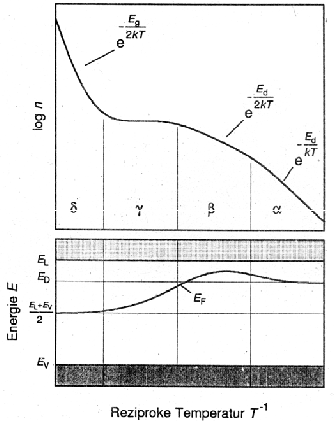
\includegraphics[width=.5\textwidth]{./img/itscomplicated.pdf}
	\caption[Electron density of a n-doped semiconductor as a function of reciprocal temperature]{\textbf{Electron density of a n-doped semiconductor as a function of reciprocal temperature}}
	\label{fig:itscomplicated}
\end{figure}

In total, the conductivity $\sigma = en\mu$ takes on a complicated behavior, depicted in \autoref{fig:itscomplicated}.

\section{BCS Theory of Superconductivity}
To describe the phenomenon of superconductivity, two electrons travelling through the lattice are considered to be in a common state, called \textit{cooper pairs}.
The first electron polarizes the lattice by interacting with the positively charged nuclei and attracting them.
This leads to a concentration of positive charge along the trajectory of the first electron.
Since the nuclei are relatively heavy, they only return to their point of equilibrium very slowly and thus create an energetically more favorable path for the second electron to travel along.
As a result of this indirect coupling between these two electrons, they are bound to a single cooper pair.
Both electrons now possess a lowered energy which can overcompensate the Coulomb repelling between them, as long as they are far enough apart.

Detailed calculations yield that their spins and momenta have to be antiparallel.
As a result of no net momentum, the cooper pair does not have kinetic energy.
Therefore, it will not be able to release energy by scattering with the lattice, effectively travelling resistance-free.
Hence, the creation of a cooper pair is an interaction with virtual phonons.

However, the bond of a cooper pair can be broken if the thermal energy of the lattice $k_\text{B}T$ exceeds the so called \textit{critical temperature} $T_\text{c}$ or if a high enough current flows through the material.

\subsection{The Meißner-Ochsenfeld Effect}
Below their critical temperatures, superconductors are not only ideal conductors but also ideal diamagnets.
They expel an external magnetic field $B_\text{ext}$ during their transition to a superconducting phase, as long as the external field does not exceed the so called \textit{critical field}.
This expulsion is a result of induced surface currents creating an opposing field.

\subsection{Classification of Superconductors}
\begin{itemize}
	\item \textbf{Superconductors of the 1st kind} expel external fields completely for $B<B_\text{c}$.
	\item \textbf{Superconductors of the 2nd kind} only expel external fields completely for $B<B_{c1}<B_c$ and graudally transition to a normally conducting state for  $B>B_{c2}>B_c$.
	A state in which an external B-field penetrates the material partially for $B_{c1}<B<B_{c2}$ is called the \textit{Shubnikov phase}.
	The external field then penetrates the superconductor in so called \textit{flux tubes}.
\end{itemize}
